\section{TEST CASES AND RESULTS}
The images below each test case show the result and the log of the automatic test respectively.
\subsection{Fleet manager: Login}
\begin{center}
	\begin{tabular} { | m{3.5cm} | m{9.5cm} | }
		\hline
		\textbf{Test Case ID} & \#1\\
		\hline
		\textbf{Test Case Name} & Fleet manager: Login\\
		\hline
		\textbf{User Story ID} & \#1\\
		\hline
		\textbf{Actor Involved} & Fleet manager\\
		\hline
		\textbf{Precondition} & Fleet manager's credentials are saved into the database.\\
		\hline
		\textbf{Main Path} & 
		\begin{enumerate}
			\item Open website homepage.
			\item Click on \textit{Fleet managers \& Bus drivers} button.
			\item Enter \textit{Username} (e.g. "Ste") and \textit{Password} (e.g. "abcdefg") in the corresponding fields.
			\item Click on \textit{Login} button.
		\end{enumerate}\\
		\hline
		\textbf{Expected Result} & Fleet manager is able to view his/her personal page.\\
		\hline
		\textbf{Manual testing} & PASSED\\
		\hline
	\end{tabular}
\end{center}

\begin{figure}[H]
	\centering
	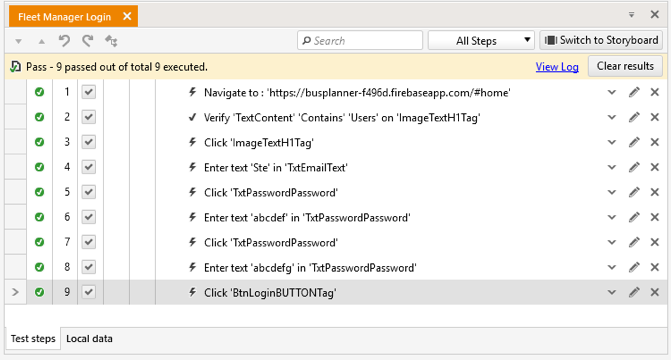
\includegraphics[width=14cm]{FmLogin1}
\end{figure}
\begin{figure}[H]
	\centering
	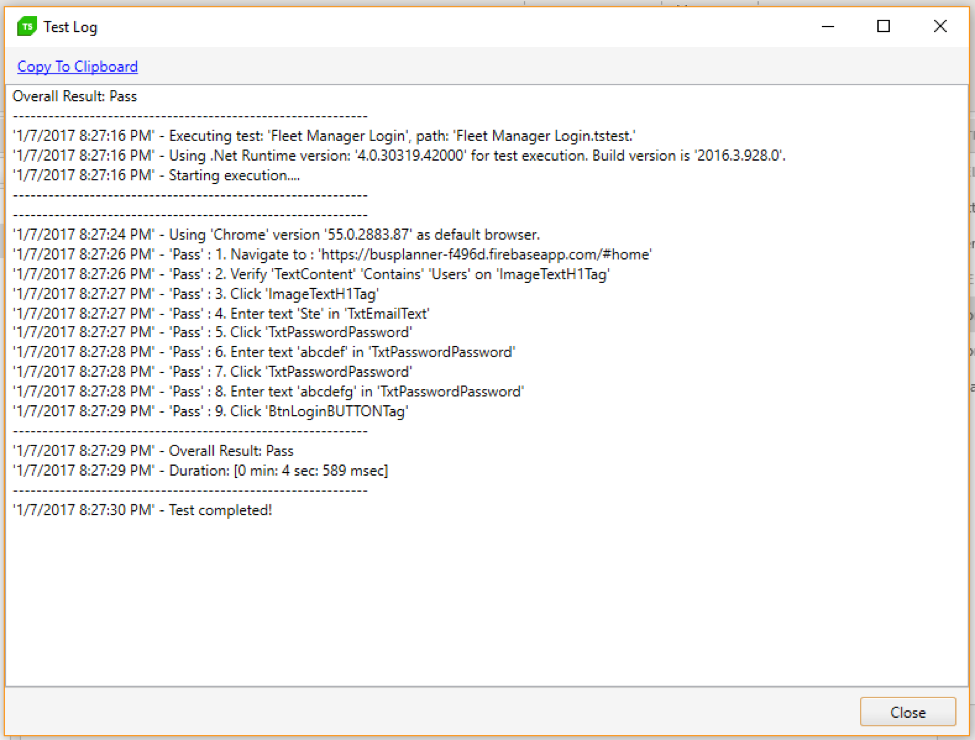
\includegraphics[width=14cm]{FmLogin2}
\end{figure}
\newpage
\subsection{Fleet manager: Logout}
\begin{center}
	\begin{tabular} { | m{3.5cm} | m{9.5cm} | }
		\hline
		\textbf{Test Case ID} & \#2\\
		\hline
		\textbf{Test Case Name} & Fleet manager: Logout\\
		\hline
		\textbf{User Story ID} & - \\
		\hline
		\textbf{Actor Involved} & Fleet manager\\
		\hline
		\textbf{Precondition} & Fleet manager is logged into the system.\\
		\hline
		\textbf{Main Path} & 
		\begin{enumerate}
			\item Click on \textit{Logout} button in the upper right corner of the page.
		\end{enumerate}\\
		\hline
		\textbf{Expected Result} & Fleet manager is able to view the website page with the login form.\\
		\hline
		\textbf{Manual testing} & PASSED\\
		\hline
	\end{tabular}
\end{center}
\begin{figure}[H]
	\centering
	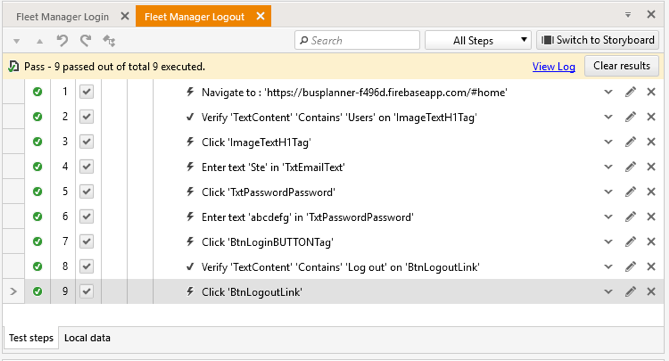
\includegraphics[width=14cm]{FmLogout1}
\end{figure}
\begin{figure}[H]
	\centering
	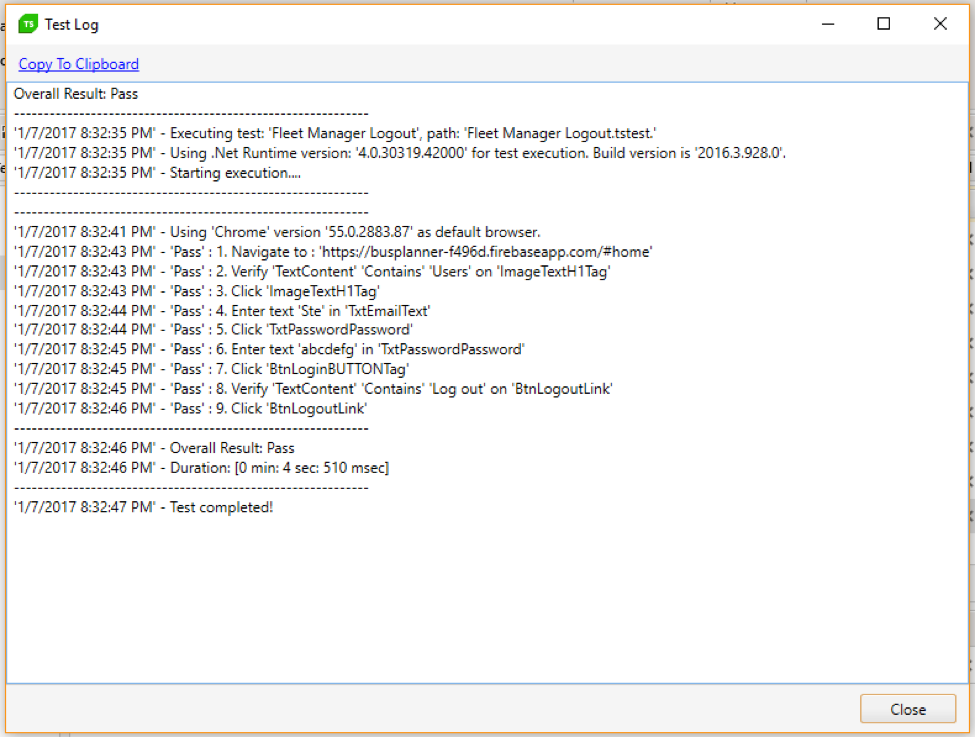
\includegraphics[width=14cm]{FmLogout2}
\end{figure}
\newpage
\subsection{Fleet manager: Add bus}
\begin{center}
	\begin{tabular} { | m{3.5cm} | m{9.5cm} | }
		\hline
		\textbf{Test Case ID} & \#3\\
		\hline
		\textbf{Test Case Name} & Fleet manager: Add bus\\
		\hline
		\textbf{User Story ID} & \#2 \\
		\hline
		\textbf{Actor Involved} & Fleet manager\\
		\hline
		\textbf{Precondition} & Fleet manager is logged into the system.\\
		\hline
		\textbf{Main Path} & 
		\begin{enumerate}
			\item Click on \textit{Buses} button from the fleet manager's personal page.
			\item Click on \textit{ADD BUS} button at the bottom of the page.
			\item Enter the bus' information.
			\item Click on \textit{Submit} button.
		\end{enumerate}\\
		\hline
		\textbf{Expected Result} & Fleet manager is able to see the bus he/she just added at the bottom of the buses list.\\
		\hline
		\textbf{Manual testing} & PASSED\\
		\hline
	\end{tabular}
\end{center}
\begin{figure}[H]
\centering
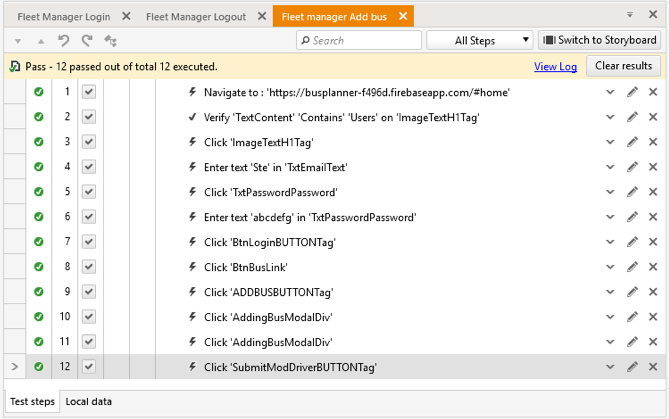
\includegraphics[width=14cm]{FmAddBus1}
\end{figure}
\begin{figure}[H]
\centering
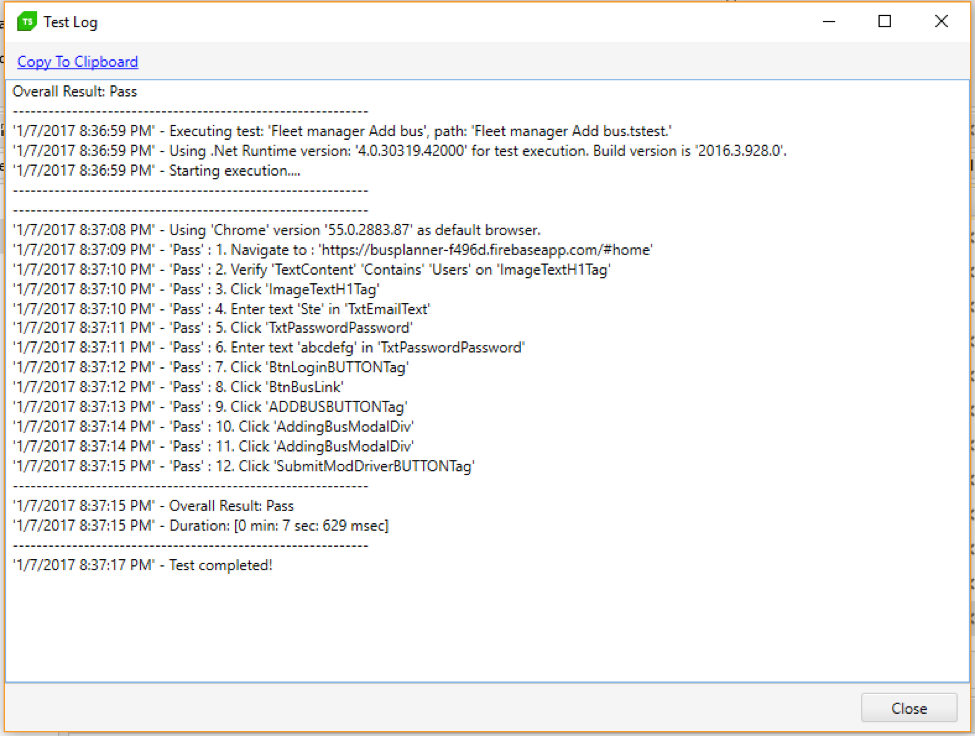
\includegraphics[width=14cm]{FmAddBus2}
\end{figure}
\newpage
\subsection{Fleet manager: Modify bus}
\begin{center}
	\begin{tabular} { | m{3.5cm} | m{9.5cm} | }
		\hline
		\textbf{Test Case ID} & \#4\\
		\hline
		\textbf{Test Case Name} & Fleet manager: Modify bus\\
		\hline
		\textbf{User Story ID} & \#2 \\
		\hline
		\textbf{Actor Involved} & Fleet manager\\
		\hline
		\textbf{Precondition} & Fleet manager is logged into the system.\\
		\hline
		\textbf{Main Path} & 
		\begin{enumerate}
			\item Click on \textit{Buses} button from the fleet manager's personal page.
			\item Click on \textit{Modify} next to the bus to be modified.
			\item Enter the new values in the corresponding fields.
			\item Click on \textit{Submit} button.
		\end{enumerate}\\
		\hline
		\textbf{Expected Result} & The bus' information is modified and the fleet manager can see the new values by clicking on \textit{Info} button next to the bus he/she modified.\\
		\hline
	\textbf{Manual testing} & PASSED\\
	\hline
\end{tabular}
\end{center}
\begin{figure}[H]
\centering
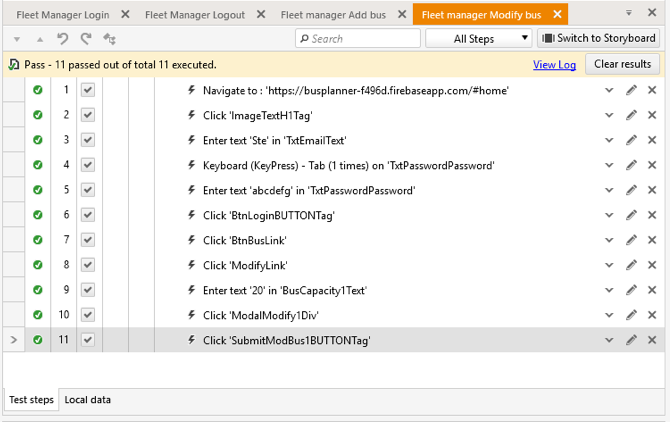
\includegraphics[width=14cm]{FmModifyBus1}
\end{figure}
\begin{figure}[H]
\centering
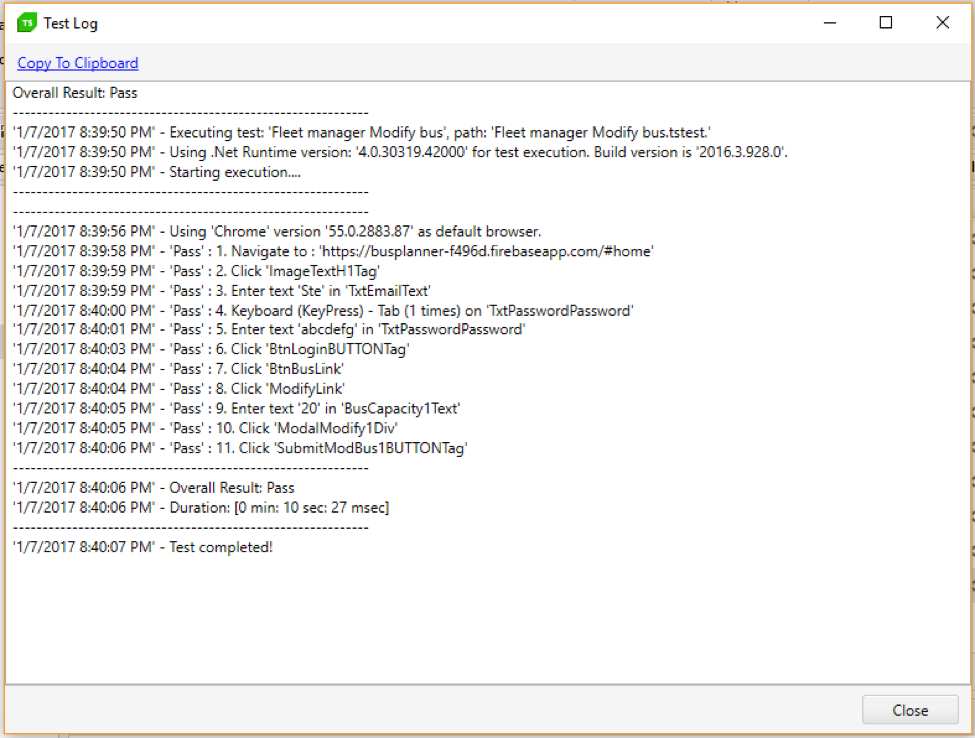
\includegraphics[width=14cm]{FmModifyBus2}
\end{figure}
\newpage
\subsection{Fleet manager: Remove bus}
\begin{center}
	\begin{tabular} { | m{3.5cm} | m{9.5cm} | }
		\hline
		\textbf{Test Case ID} & \#5\\
		\hline
		\textbf{Test Case Name} & Fleet manager: Remove bus\\
		\hline
		\textbf{User Story ID} & \#2 \\
		\hline
		\textbf{Actor Involved} & Fleet manager\\
		\hline
		\textbf{Precondition} & Fleet manager is logged into the system.\\
		\hline
		\textbf{Main Path} & 
		\begin{enumerate}
			\item Click on \textit{Buses} button from the fleet manager's personal page.
			\item Click on \textit{Delete} next to the bus to be removed.
			\item Click on \textit{Delete} button in the form that is going to appear.
		\end{enumerate}\\
		\hline
		\textbf{Expected Result} & Fleet manager is able to view the list of buses without the one he/she just removed.\\
		\hline
	\textbf{Manual testing} & PASSED\\
	\hline
\end{tabular}
\end{center}
\begin{figure}[H]
\centering
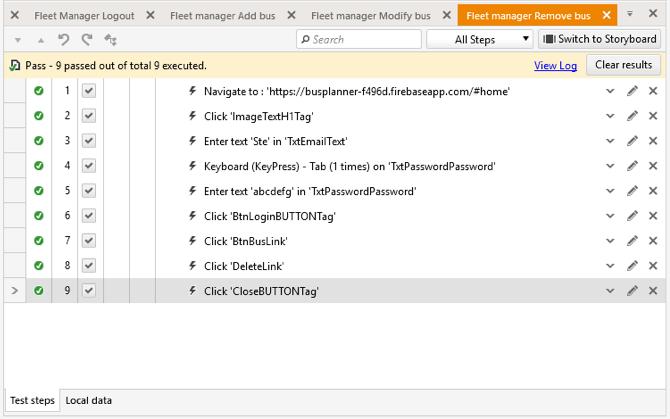
\includegraphics[width=14cm]{FmRemoveBus1}
\end{figure}
\begin{figure}[H]
\centering
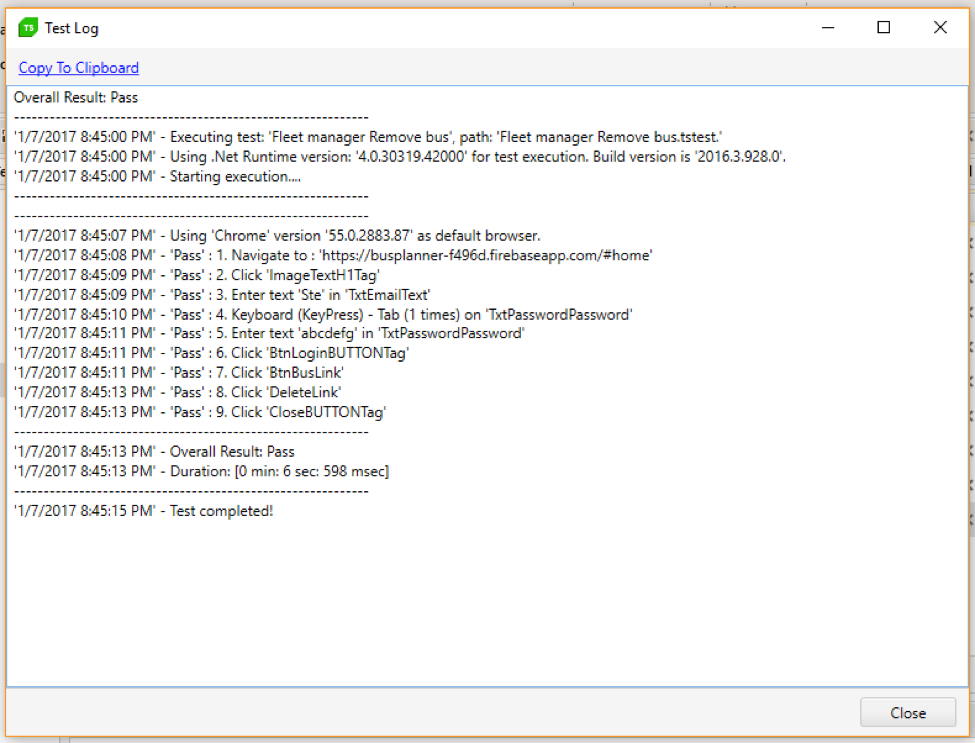
\includegraphics[width=14cm]{FmRemoveBus2}
\end{figure}
\newpage
\subsection{Fleet manager: Add driver}
\begin{center}
	\begin{tabular} { | m{3.5cm} | m{9.5cm} | }
		\hline
		\textbf{Test Case ID} & \#6\\
		\hline
		\textbf{Test Case Name} & Fleet manager: Add driver\\
		\hline
		\textbf{User Story ID} & \#3 \\
		\hline
		\textbf{Actor Involved} & Fleet manager\\
		\hline
		\textbf{Precondition} & Fleet manager is logged into the system.\\
		\hline
		\textbf{Main Path} & 
		\begin{enumerate}
			\item Click on \textit{Drivers} button from the fleet manager's personal page.
			\item Click on \textit{NEW DRIVER} button at the bottom of the page.
			\item Enter the driver's information.
			\item Click on \textit{Submit} button.
		\end{enumerate}\\
		\hline
		\textbf{Expected Result} & Fleet manager is able to see the driver he/she just added at the bottom of the drivers list.\\
		\hline
	\textbf{Manual testing} & PASSED\\
	\hline
\end{tabular}
\end{center}
\begin{figure}[H]
\centering
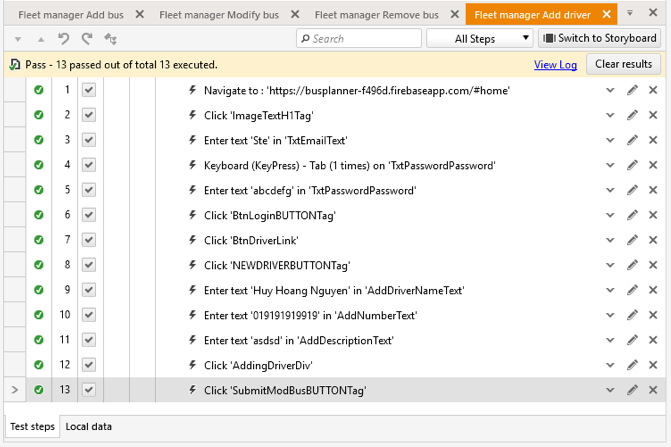
\includegraphics[width=14cm]{FmAddDriver1}
\end{figure}
\begin{figure}[H]
\centering
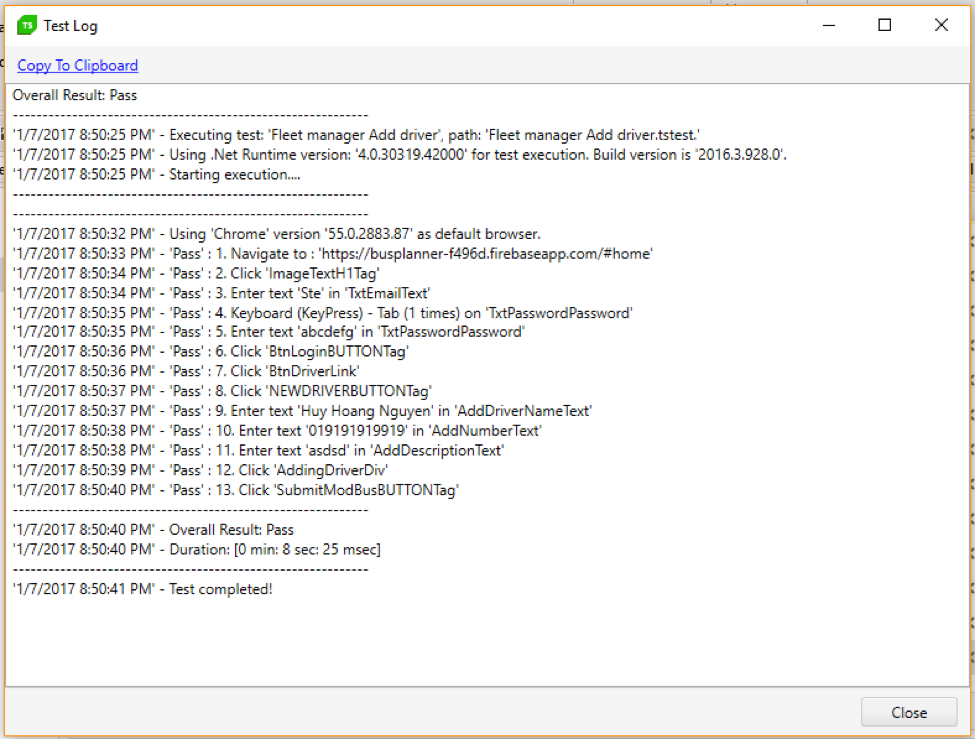
\includegraphics[width=14cm]{FmAddDriver2}
\end{figure}
\newpage
\subsection{Fleet manager: Modify driver}
\begin{center}
	\begin{tabular} { | m{3.5cm} | m{9.5cm} | }
		\hline
		\textbf{Test Case ID} & \#7\\
		\hline
		\textbf{Test Case Name} & Fleet manager: Modify driver\\
		\hline
		\textbf{User Story ID} & \#3 \\
		\hline
		\textbf{Actor Involved} & Fleet manager\\
		\hline
		\textbf{Precondition} & Fleet manager is logged into the system.\\
		\hline
		\textbf{Main Path} & 
		\begin{enumerate}
			\item Click on \textit{Drivers} button from the fleet manager's personal page.
			\item Click on \textit{Modify} next to the driver to be modified.
			\item Enter the new values in the corresponding fields.
			\item Click on \textit{Submit} button.
		\end{enumerate}\\
		\hline
		\textbf{Expected Result} & The driver's information are modified and the fleet manager can see the new values by clicking on \textit{Info} button next to the driver he/she modified.\\
		\hline
	\textbf{Manual testing} & PASSED\\
	\hline
\end{tabular}
\end{center}
\begin{figure}[H]
\centering
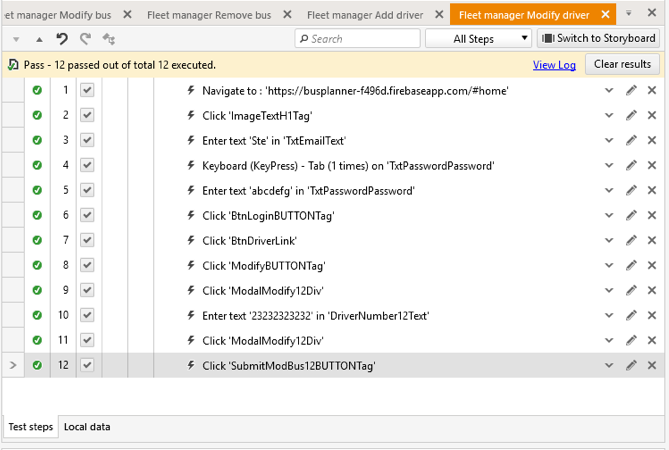
\includegraphics[width=14cm]{FmModifyDriver1}
\end{figure}

\begin{figure}[H]
\centering
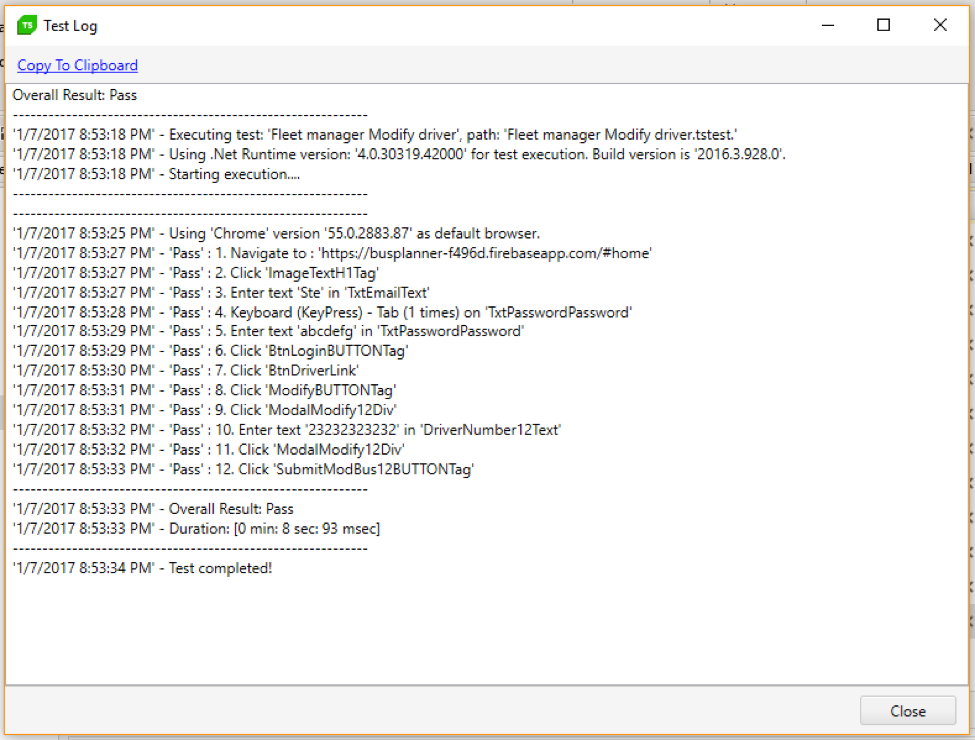
\includegraphics[width=14cm]{FmModifyDriver2}
\end{figure}
\newpage
\subsection{Fleet manager: Remove driver}
\begin{center}
	\begin{tabular} { | m{3.5cm} | m{9.5cm} | }
		\hline
		\textbf{Test Case ID} & \#8\\
		\hline
		\textbf{Test Case Name} & Fleet manager: Remove driver\\
		\hline
		\textbf{User Story ID} & \#3 \\
		\hline
		\textbf{Actor Involved} & Fleet manager\\
		\hline
		\textbf{Precondition} & Fleet manager is logged into the system.\\
		\hline
		\textbf{Main Path} & 
		\begin{enumerate}
			\item Click on \textit{Drivers} button from the fleet manager's personal page.
			\item Click on \textit{Delete} next to the driver to be removed.
			\item Click on \textit{Delete} button in the form that is going to appear.
		\end{enumerate}\\
		\hline
		\textbf{Expected Result} & Fleet manager is able to view the list of drivers without the one he/she just removed.\\
		\hline
	\textbf{Manual testing} & PASSED\\
	\hline
\end{tabular}
\end{center}
\begin{figure}[H]
\centering
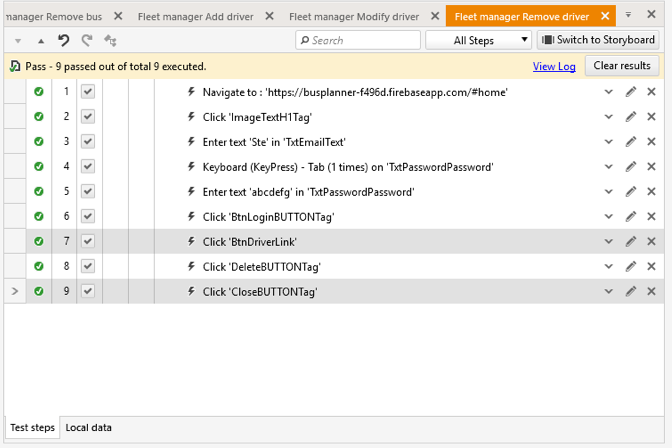
\includegraphics[width=14cm]{FmRemoveDriver1}
\end{figure}
\begin{figure}[H]
\centering
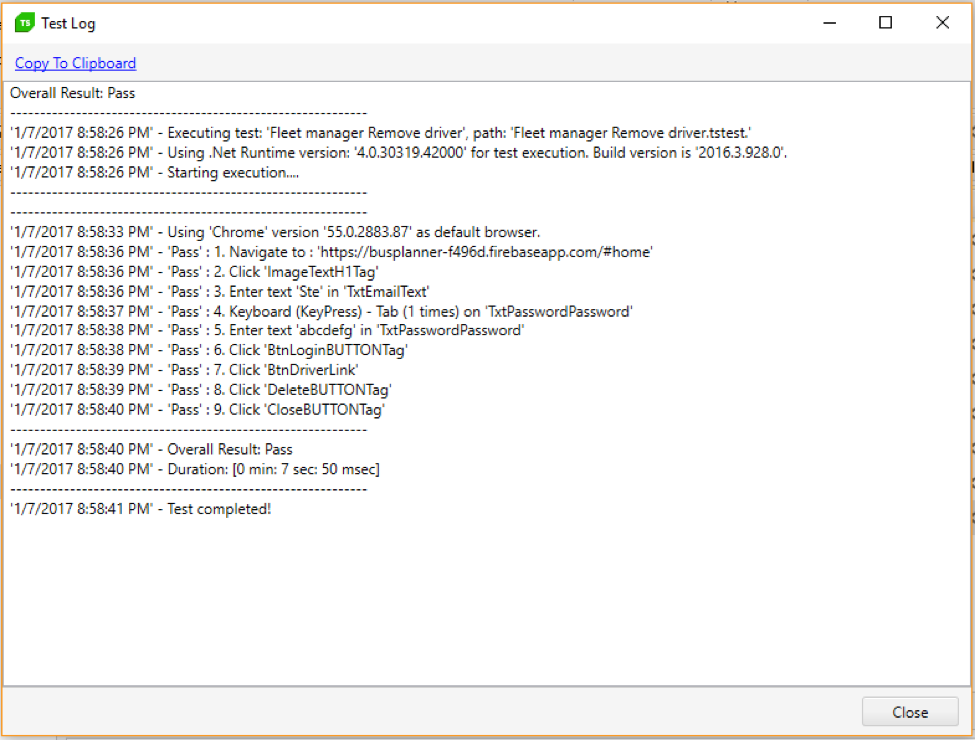
\includegraphics[width=14cm]{FmRemoveDriver2}
\end{figure}
\newpage
\subsection{Fleet manager: View  user requests}
\begin{center}
	\begin{tabular} { | m{3.5cm} | m{9.5cm} | }
		\hline
		\textbf{Test Case ID} & \#9\\
		\hline
		\textbf{Test Case Name} & Fleet manager: View user requests on a map\\
		\hline
		\textbf{User Story ID} & \#4 \\
		\hline
		\textbf{Actor Involved} & Fleet manager\\
		\hline
		\textbf{Precondition} & Fleet manager is logged into the system.\\
		\hline
		\textbf{Main Path} & 
		\begin{enumerate}
			\item Click on \textit{User Requests} button from the fleet manager's personal page.
		\end{enumerate}\\
		\hline
		\textbf{Expected Result} & Fleet manager is able to view the user requests on a map.\\
		\hline
	\textbf{Manual testing} & PASSED\\
	\hline
\end{tabular}
\end{center}
\begin{figure}[H]
\centering
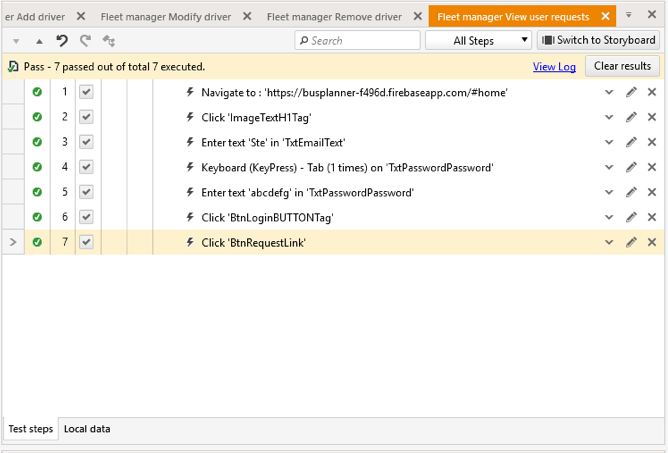
\includegraphics[width=14cm]{FmViewUserRequests1}
\end{figure}
\begin{figure}[H]
\centering
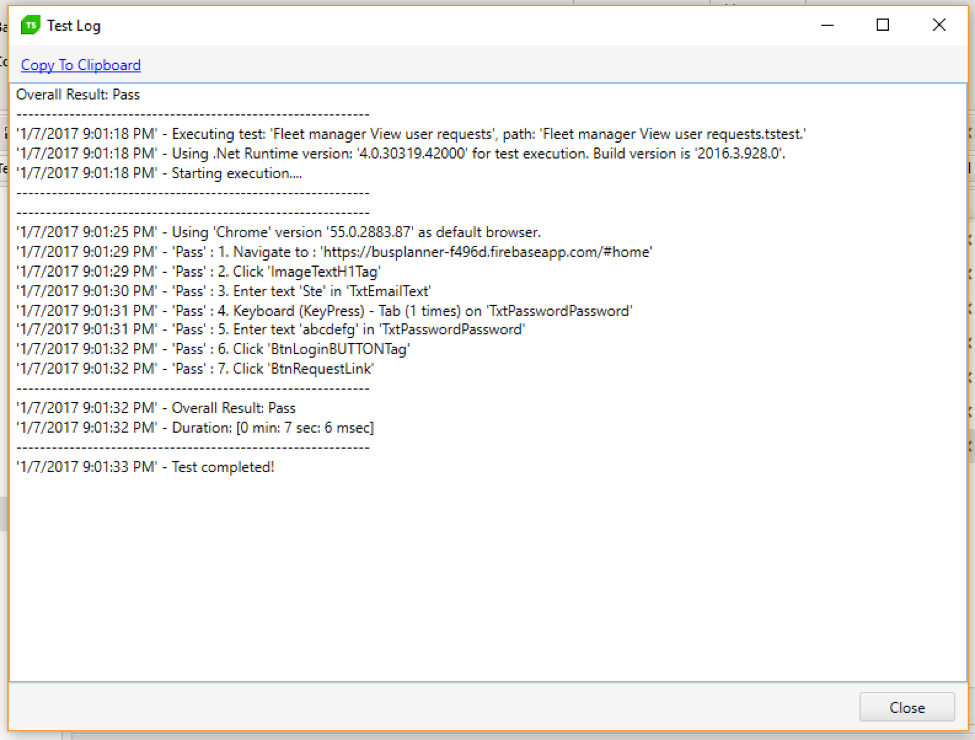
\includegraphics[width=14cm]{FmViewUserRequests2}
\end{figure}
\newpage
\subsection{Fleet manager: View previous user requests}
\begin{center}
	\begin{tabular} { | m{3.5cm} | m{9.5cm} | }
		\hline
		\textbf{Test Case ID} & \#10\\
		\hline
		\textbf{Test Case Name} & Fleet manager: View previous user requests\\
		\hline
		\textbf{User Story ID} & \#5 \\
		\hline
		\textbf{Actor Involved} & Fleet manager\\
		\hline
		\textbf{Precondition} & Fleet manager is logged into the system.\\
		\hline
		\textbf{Main Path} & 
		\begin{enumerate}
			\item Click on \textit{User Requests} button from the fleet manager's personal page.
		\end{enumerate}\\
		\hline
		\textbf{Expected Result} & Fleet manager is able to view the past user requests in a table, with all the related information.\\
		\hline
	\textbf{Manual testing} & PASSED\\
	\hline
\end{tabular}
\end{center}
\begin{figure}[H]
\centering
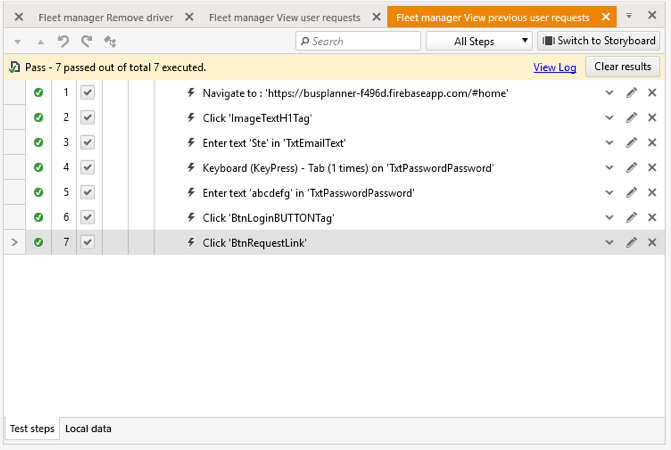
\includegraphics[width=14cm]{FmViewPreviousUserRequests1}
\end{figure}
\begin{figure}[H]
\centering
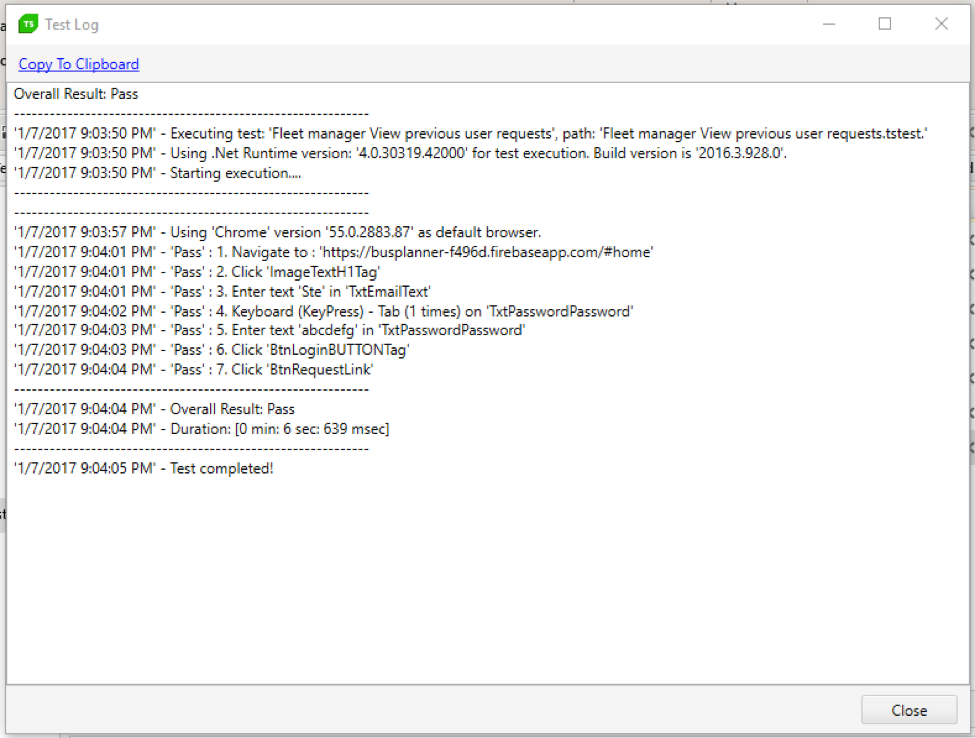
\includegraphics[width=14cm]{FmViewPreviousUserRequests2}
\end{figure}
\newpage
\subsection{Fleet manager: Get buses location}
\begin{center}
	\begin{tabular} { | m{3.5cm} | m{9.5cm} | }
		\hline
		\textbf{Test Case ID} & \#11\\
		\hline
		\textbf{Test Case Name} & Fleet manager: Get buses location\\
		\hline
		\textbf{User Story ID} & \#6 \\
		\hline
		\textbf{Actor Involved} & Fleet manager\\
		\hline
		\textbf{Precondition} & Fleet manager is logged into the system.\\
		\hline
		\textbf{Main Path} & 
		\begin{enumerate}
			\item Click on \textit{Buses} button from the fleet manager's personal page.
		\end{enumerate}\\
		\hline
		\textbf{Expected Result} & Fleet manager is able to see a map showing the location of all the buses of the company.\\
		\hline
	\textbf{Manual testing} & PASSED\\
	\hline
\end{tabular}
\end{center}
\begin{figure}[H]
\centering
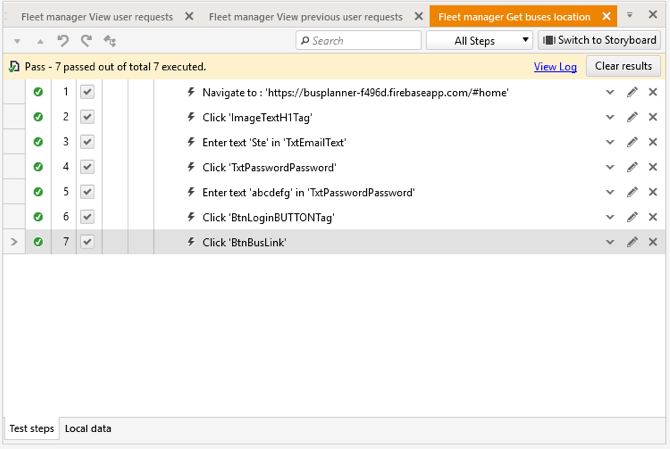
\includegraphics[width=14cm]{FmGetBusesLocation1}
\end{figure}
\begin{figure}[H]
\centering
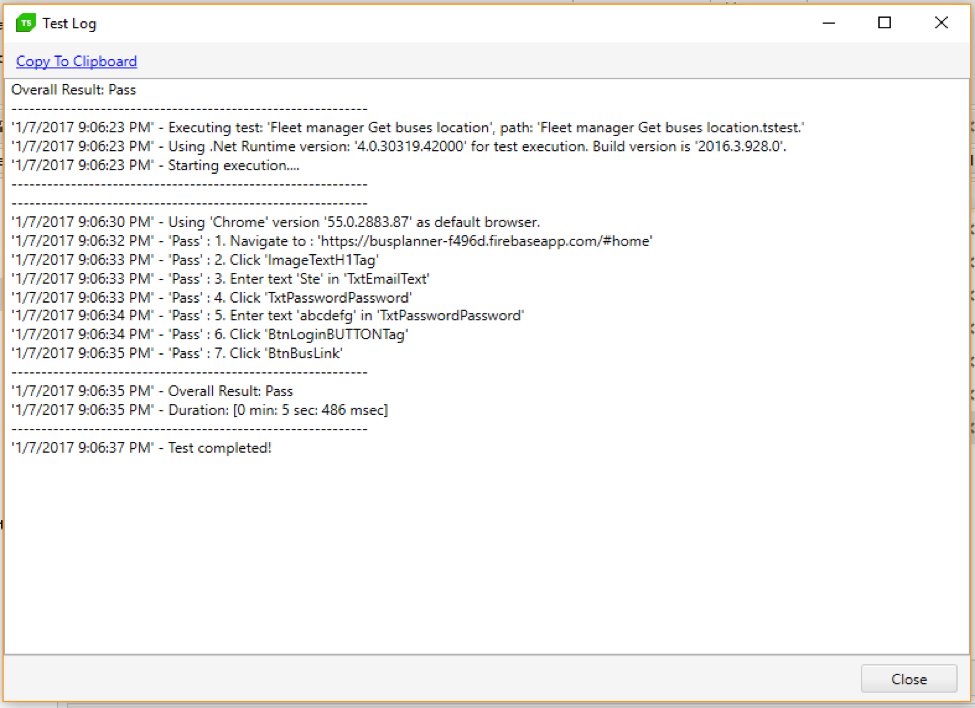
\includegraphics[width=14cm]{FmGetBusesLocation2}
\end{figure}
\newpage
\subsection{Fleet manager: View routes and stops utilization}
\begin{center}
	\begin{tabular} { | m{3.5cm} | m{9.5cm} | }
		\hline
		\textbf{Test Case ID} & \#12\\
		\hline
		\textbf{Test Case Name} & Fleet manager: View routes and stops utilization\\
		\hline
		\textbf{User Story ID} & \#7 \\
		\hline
		\textbf{Actor Involved} & Fleet manager\\
		\hline
		\textbf{Precondition} & Fleet manager is logged into the system.\\
		\hline
		\textbf{Main Path} & 
		\begin{enumerate}
			\item Click on \textit{Statistics} button from the fleet manager's personal page.
		\end{enumerate}\\
		\hline
		\textbf{Expected Result} & Fleet manager is able to see a chart showing the utilization of all the routes of the company and a chart showing the utilization of the five stops mostly used.\\
		\hline
	\textbf{Manual testing} & PASSED\\
	\hline
\end{tabular}
\end{center}
\begin{figure}[H]
\centering
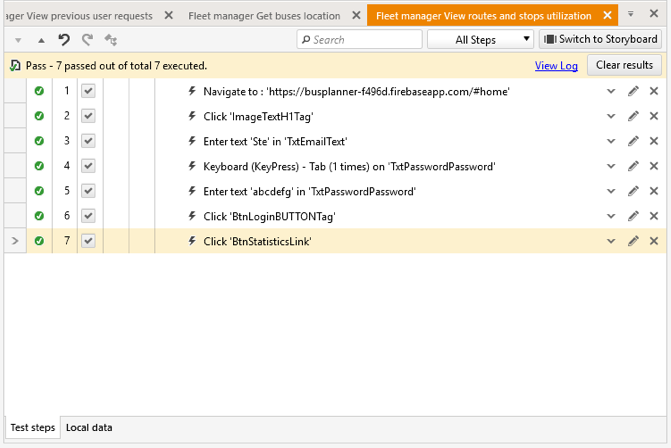
\includegraphics[width=14cm]{FmRoutesUtilization1}
\end{figure}
\begin{figure}[H]
\centering
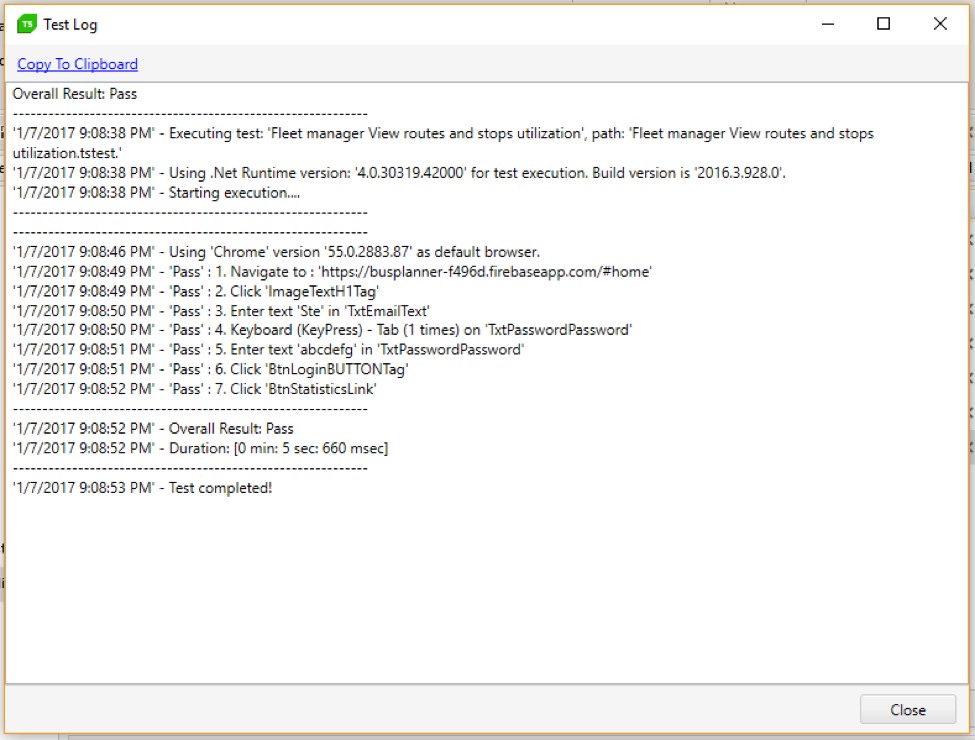
\includegraphics[width=14cm]{FmRoutesUtilization2}
\end{figure}
\newpage
\subsection{Fleet manager: View routes}
\begin{center}
	\begin{tabular} { | m{3.5cm} | m{9.5cm} | }
		\hline
		\textbf{Test Case ID} & \#13\\
		\hline
		\textbf{Test Case Name} & Fleet manager: View routes \\
		\hline
		\textbf{User Story ID} & - \\
		\hline
		\textbf{Actor Involved} & Fleet manager\\
		\hline
		\textbf{Precondition} & Fleet manager is logged into the system.\\
		\hline
		\textbf{Main Path} & 
		\begin{enumerate}
			\item Click on \textit{Routes} button from the fleet manager's personal page.
			\item By clicking on a route the map will change, showing that specific route.
		\end{enumerate}\\
		\hline
		\textbf{Expected Result} & Fleet manager is able to see the company's routes:
		\begin{itemize}
			\item On the left there is the routes' list.
			\item On the right there is a map showing the bus stops location for each route. 
		\end{itemize}\\
		\hline
	\textbf{Manual testing} & PASSED\\
	\hline
\end{tabular}
\end{center}
\begin{figure}[H]
\centering
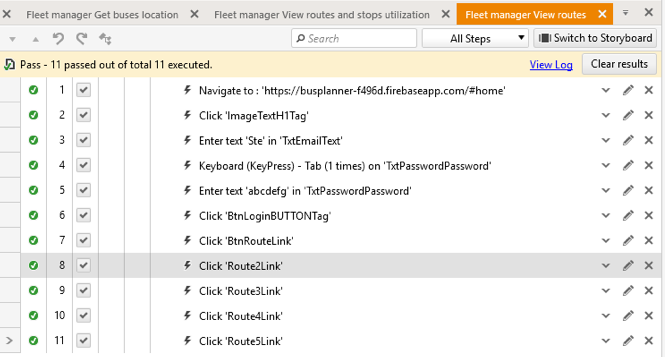
\includegraphics[width=14cm]{FmViewRoutes1}
\end{figure}
\begin{figure}[H]
\centering
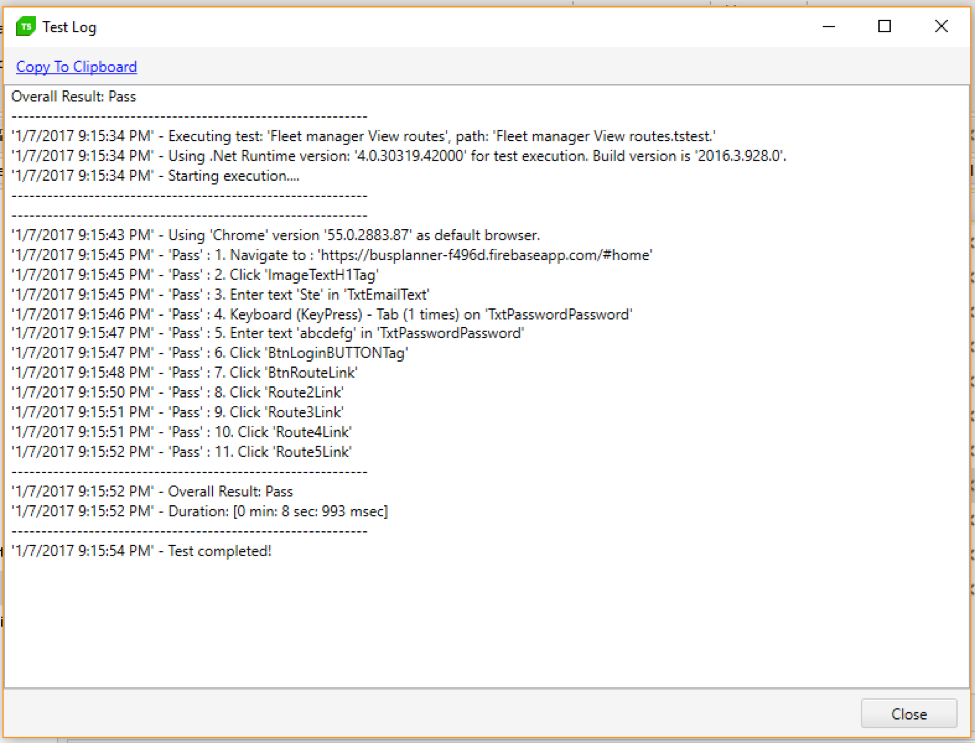
\includegraphics[width=14cm]{FmViewRoutes2}
\end{figure}
\newpage
\subsection{Fleet manager: Add route}
\begin{center}
	\begin{tabular} { | m{3.5cm} | m{9.5cm} | }
		\hline
		\textbf{Test Case ID} & \#14\\
		\hline
		\textbf{Test Case Name} & Fleet manager: Add route\\
		\hline
		\textbf{User Story ID} & \#8 \\
		\hline
		\textbf{Actor Involved} & Fleet manager\\
		\hline
		\textbf{Precondition} & Fleet manager is logged into the system.\\
		\hline
		\textbf{Main Path} & 
		\begin{enumerate}
			\item Click on \textit{Routes} button from the fleet manager's personal page.
			\item Click on \textit{ADD ROUTE} button at the bottom of the page.
			\item Enter the route's name and choose the route stops by clicking directly on the map after inserting the name of the stop.
			\item Click on \textit{Submit} button.
		\end{enumerate}\\
		\hline
		\textbf{Expected Result} & Fleet manager is able to see the route he/she just added at the bottom of the routes list.\\
		\hline
	\textbf{Manual testing} & PASSED\\
	\hline
\end{tabular}
\end{center}
\begin{figure}[H]
\centering
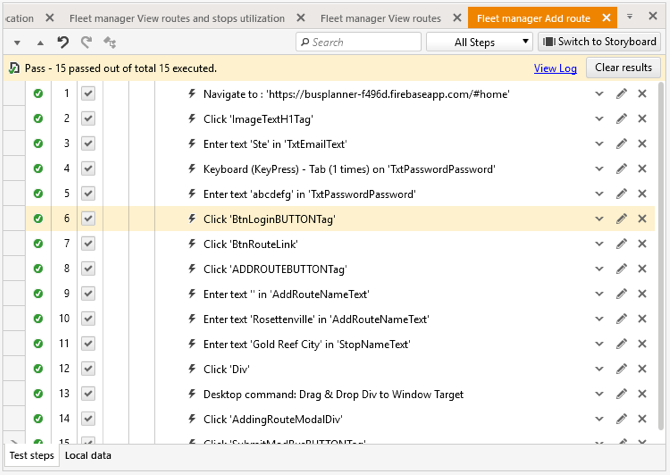
\includegraphics[width=14cm]{FmAddRoute1}
\end{figure}
\begin{figure}[H]
\centering
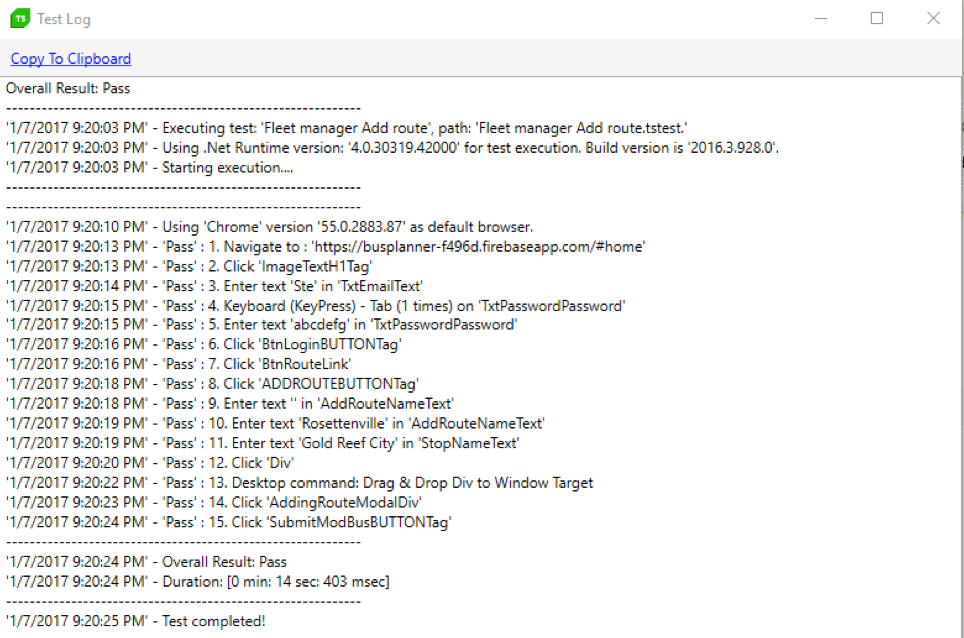
\includegraphics[width=14cm]{FmAddRoute2}
\end{figure}
\newpage
\subsection{Fleet manager: Remove route}
\begin{center}
	\begin{tabular} { | m{3.5cm} | m{9.5cm} | }
		\hline
		\textbf{Test Case ID} & \#15\\
		\hline
		\textbf{Test Case Name} & Fleet manager: Remove route\\
		\hline
		\textbf{User Story ID} & \#8 \\
		\hline
		\textbf{Actor Involved} & Fleet manager\\
		\hline
		\textbf{Precondition} & Fleet manager is logged into the system.\\
		\hline
		\textbf{Main Path} & 
		\begin{enumerate}
			\item Click on \textit{Routes} button from the fleet manager's personal page.
			\item Click on \textit{X} button next to the route to be removed.
			\item Click on \textit{OK} button in the form that is going to appear.
		\end{enumerate}\\
		\hline
		\textbf{Expected Result} & Fleet manager is able to view the list of drivers without the one he/she just removed.\\
		\hline
	\textbf{Manual testing} & PASSED\\
	\hline
\end{tabular}
\end{center}
\begin{figure}[H]
\centering
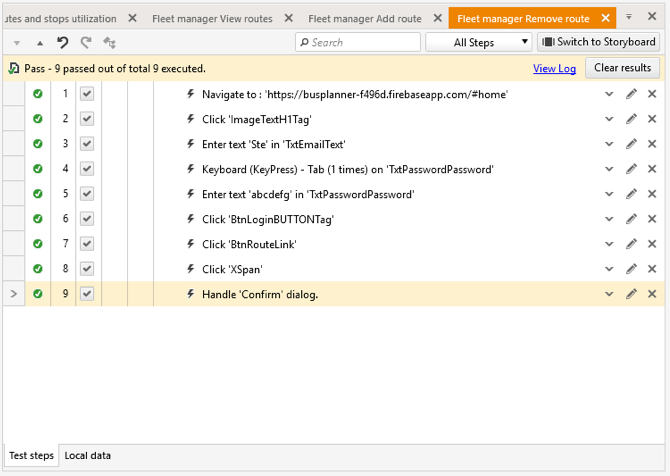
\includegraphics[width=14cm]{FmRemoveRoute1}
\end{figure}
\begin{figure}[H]
\centering
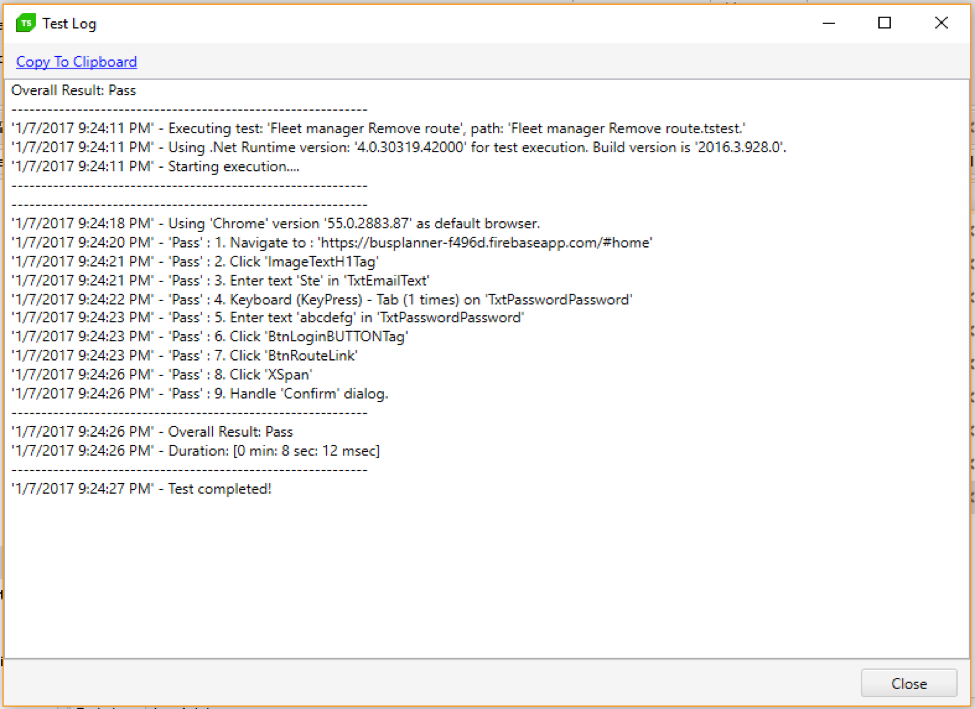
\includegraphics[width=14cm]{FmRemoveRoute2}
\end{figure}
\newpage
\subsection{Fleet manager: Back to homepage}
\begin{center}
	\begin{tabular} { | m{3.5cm} | m{9.5cm} | }
		\hline
		\textbf{Test Case ID} & \#16\\
		\hline
		\textbf{Test Case Name} & Fleet manager: Back to homepage\\
		\hline
		\textbf{User Story ID} & - \\
		\hline
		\textbf{Actor Involved} & Fleet manager\\
		\hline
		\textbf{Precondition} & Fleet manager is logged into the system.\\
		\hline
		\textbf{Main Path} & 
		\begin{enumerate}
			\item Click on \textit{BusPlanner} or on the BusPlanner logo in the upper left corner of any page.
		\end{enumerate}\\
		\hline
		\textbf{Expected Result} & Fleet manager is able to view his/her personal page.\\
		\hline
	\textbf{Manual testing} & PASSED\\
	\hline
\end{tabular}
\end{center}
\begin{figure}[H]
\centering
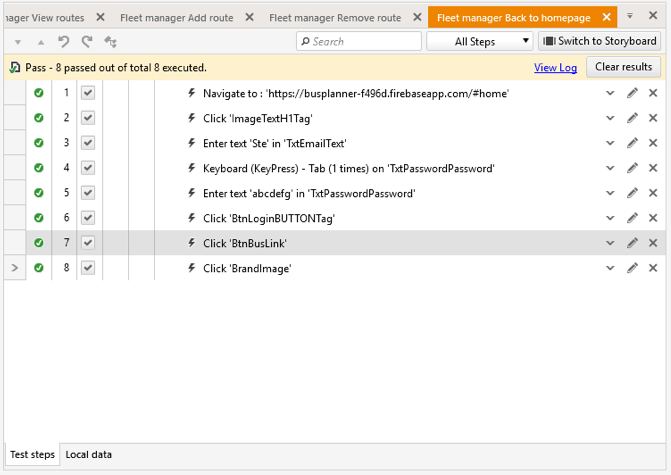
\includegraphics[width=14cm]{FmHomepage1}
\end{figure}
\begin{figure}[H]
\centering
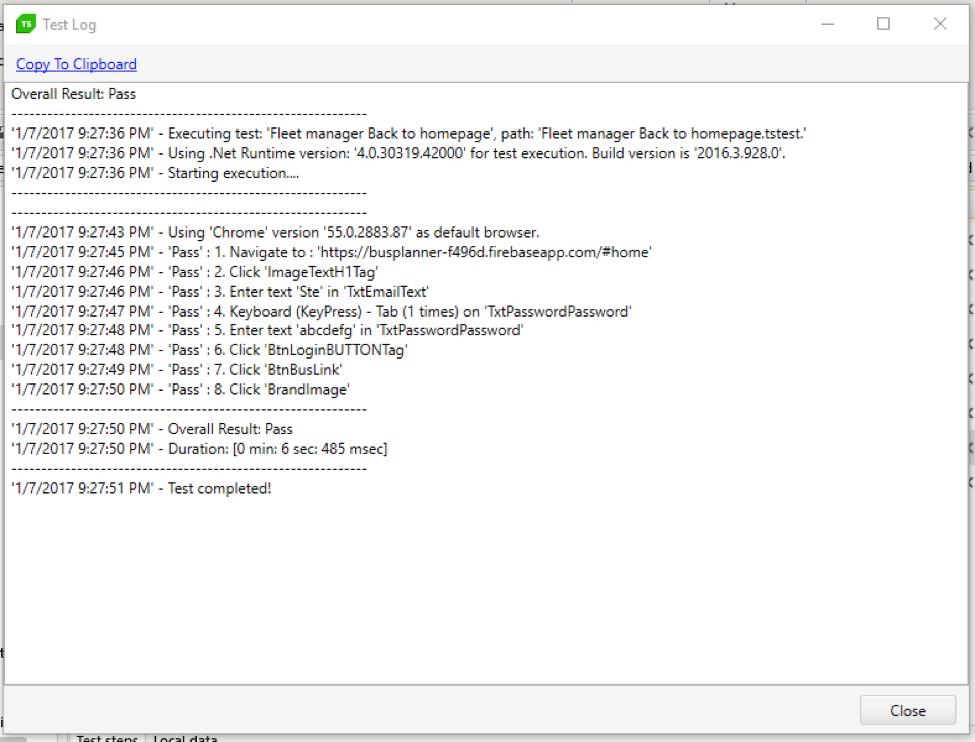
\includegraphics[width=14cm]{FmHomepage2}
\end{figure}
\newpage
\subsection{Bus driver: Login}
\begin{center}
	\begin{tabular} { | m{3.5cm} | m{9.5cm} | }
		\hline
		\textbf{Test Case ID} & \#17\\
		\hline
		\textbf{Test Case Name} & Bus driver: Login\\
		\hline
		\textbf{User Story ID} & \#9\\
		\hline
		\textbf{Actor Involved} & Bus driver\\
		\hline
		\textbf{Precondition} & Bus driver's credentials are saved into the database.\\
		\hline
		\textbf{Main Path} & 
		\begin{enumerate}
			\item Open website homepage.
			\item Click on \textit{Fleet managers \& Bus drivers} button.
			\item Enter \textit{Username} (e.g. "Albi") and \textit{Password} (e.g. "que123rty456") in the corresponding fields.
			\item Click on \textit{Login} button.
		\end{enumerate}\\
		\hline
		\textbf{Expected Result} & Bus driver is able to view his/her personal page.\\
		\hline
\textbf{Manual testing} & PASSED\\
\hline
\end{tabular}
\end{center}
\begin{figure}[H]
\centering
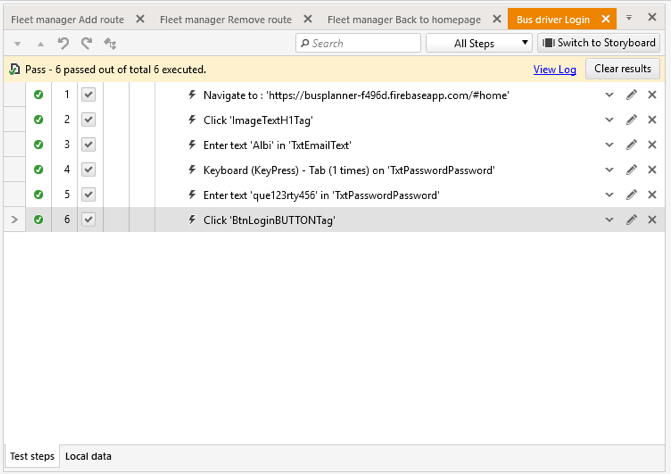
\includegraphics[width=14cm]{BdLogin1}
\end{figure}
\begin{figure}[H]
\centering
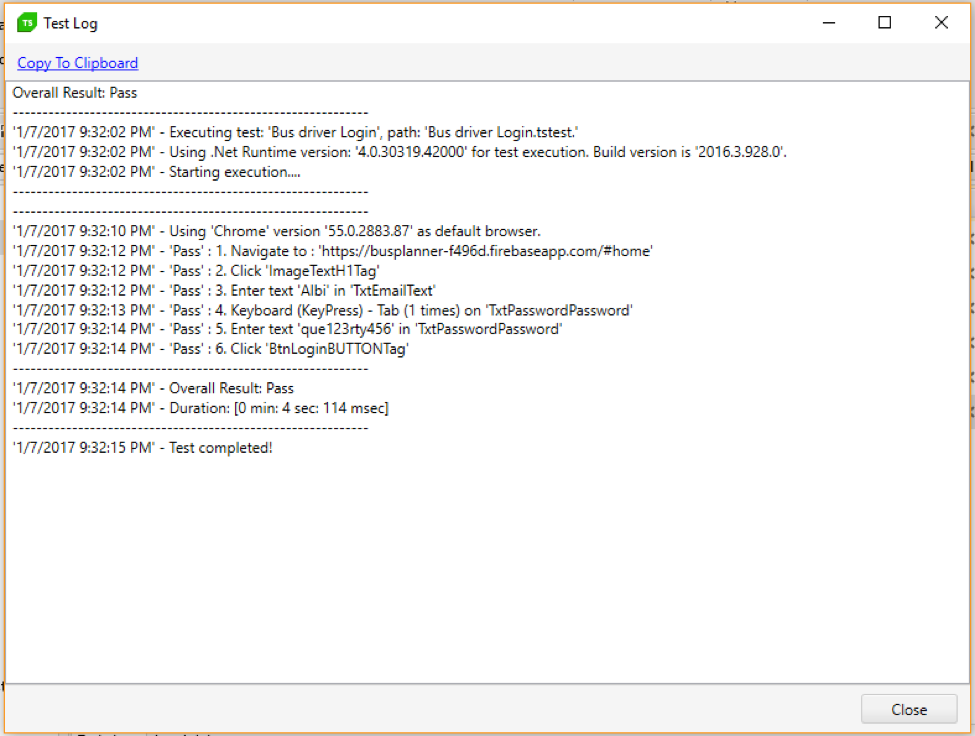
\includegraphics[width=14cm]{BdLogin2}
\end{figure}
\newpage
\subsection{Bus driver: Logout}
\begin{center}
	\begin{tabular} { | m{3.5cm} | m{9.5cm} | }
		\hline
		\textbf{Test Case ID} & \#18\\
		\hline
		\textbf{Test Case Name} & Bus driver: Logout\\
		\hline
		\textbf{User Story ID} & - \\
		\hline
		\textbf{Actor Involved} & Bus driver\\
		\hline
		\textbf{Precondition} & Bus driver is logged into the system.\\
		\hline
		\textbf{Main Path} & 
		\begin{enumerate}
			\item Click on \textit{Logout} button in the upper right corner of the page.
		\end{enumerate}\\
		\hline
		\textbf{Expected Result} & Bus driver is able to view the website page with the login form.\\
		\hline
	\textbf{Manual testing} & PASSED\\
	\hline
\end{tabular}
\end{center}
\begin{figure}[H]
\centering
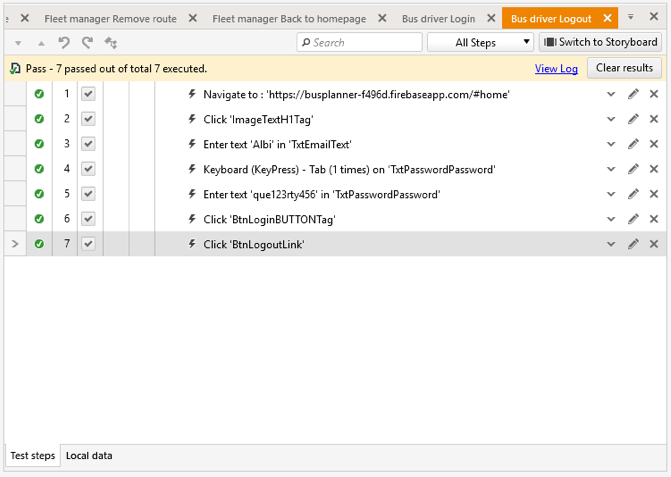
\includegraphics[width=14cm]{BdLogout1}
\end{figure}
\begin{figure}[H]
\centering
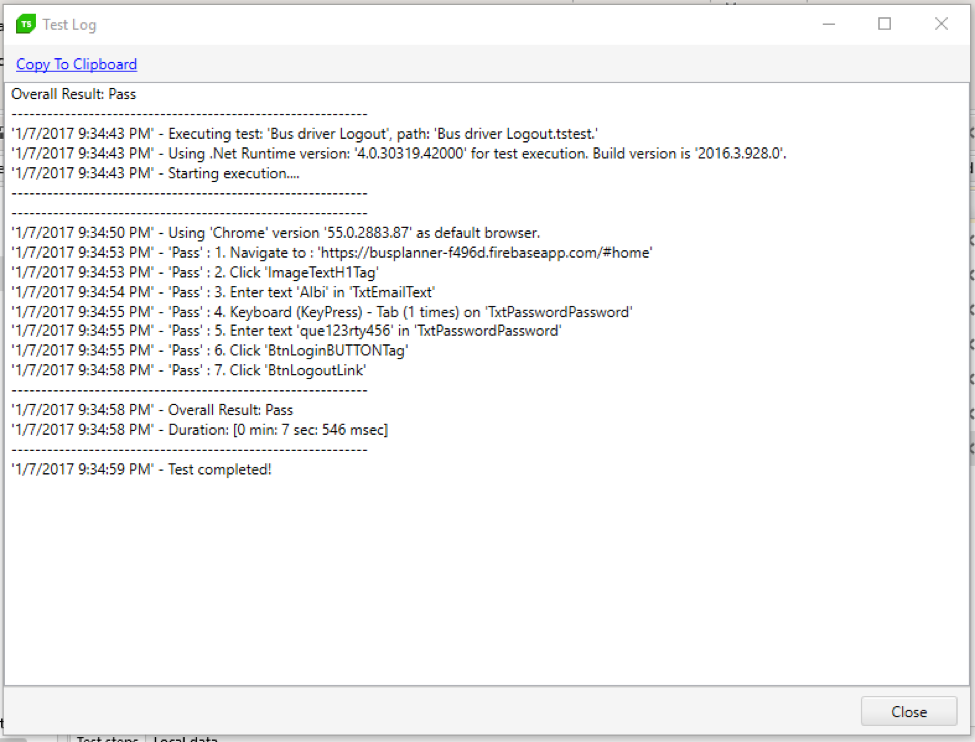
\includegraphics[width=14cm]{BdLogout2}
\end{figure}
\newpage
\subsection{Bus driver: View schedule}
\begin{center}
	\begin{tabular} { | m{3.5cm} | m{9.5cm} | }
		\hline
		\textbf{Test Case ID} & \#19\\
		\hline
		\textbf{Test Case Name} & Bus driver: View schedule\\
		\hline
		\textbf{User Story ID} & \#10 \\
		\hline
		\textbf{Actor Involved} & Bus driver\\
		\hline
		\textbf{Precondition} & Bus driver is logged into the system.\\
		\hline
		\textbf{Main Path} & 
		Bus driver can perform various actions without a specific order:
		\begin{itemize}
			\item If he/she clicks on a bus stop in the container on the left, the corresponding marker will become blue.
			\item If he/she click on a marker (red, blue or green), the name of the corresponding bus stop will appear in a window.
		\end{itemize}\\
		\hline
		\textbf{Expected Result} & Bus driver is able to see his/her schedule: 
		\begin{itemize}
			\item On the left there is a list of the bus stops he/she needs to cover, with the number of passengers that will get onto the bus at that bus stop (green number) and the number of passengers that will get off the bus at that bus stop (red number).
			\item On the right there is a map showing the bus stops location (red markers) and the user requests location (green markers).
		\end{itemize}\\
		\hline
	\textbf{Manual testing} & PASSED\\
	\hline
\end{tabular}
\end{center}
\begin{figure}[H]
\centering
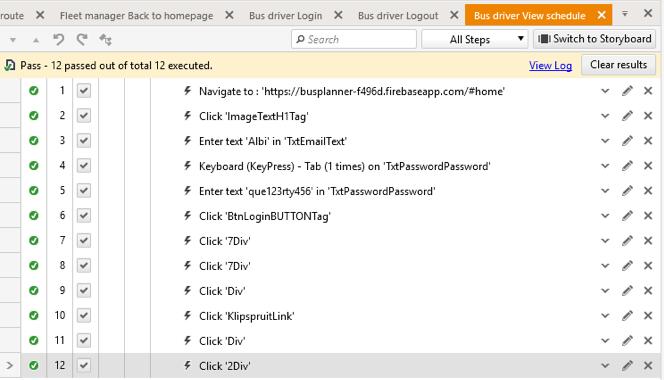
\includegraphics[width=14cm]{BdViewSchedule1}
\end{figure}
\begin{figure}[H]
\centering
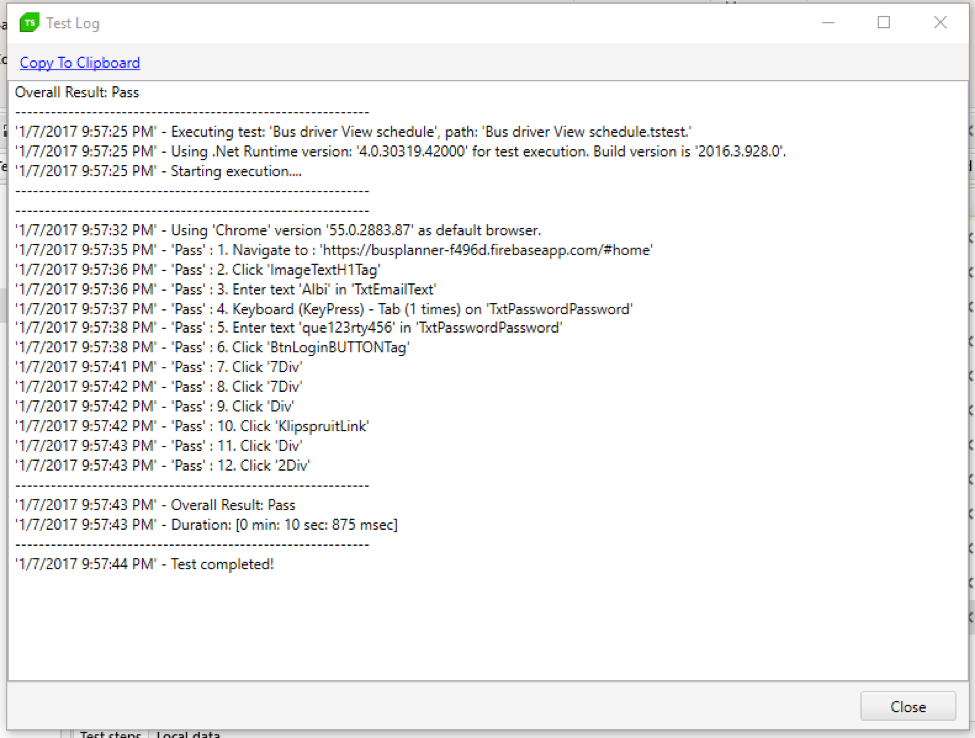
\includegraphics[width=14cm]{BdViewSchedule2}
\end{figure}